\section{Experiments on Held-Out Concurrent Streams}
\label{sec:experiments}

We evaluate end-to-end \textbf{Evid-MSED} under a strict two-stage protocol: after calibrating thresholds and confirming Stress-30\% robustness solely on \texttt{NED Validation} ($8$ events, $2{,}746$ posts), we froze \texttt{protocol\_trackB\_v1.json} containing 9 SHA-256 file digests and unlocked the unseen 24-event \texttt{NED Holdout} stream ($11{,}955$ posts) for one-shot evaluation with zero post-hoc retuning.

\subsection{Experimental Protocol and Stress-30\% Setup}
\label{sec:exp_setup}

All three splits share zero-failure image decoding ($2{,}131$ dev $+$ $1{,}950$ val $+$ $9{,}311$ holdout $= 13{,}392/13{,}392$ decoded via \texttt{PySide6}/\texttt{imageio}, zero failures) and low exact \texttt{dHash64} image duplication ($1.0\%$ dev, $2.6\%$ val, $4.5\%$ holdout). All VLM adjudication calls target \texttt{Qwen/Qwen3-VL-8B-Instruct}~\cite{bai2025qwen3vl} via SiliconFlow ($\text{temperature}=0.0$, $\text{max\_tokens}=320$, $384\text{px}$ JPEG) with immutable \texttt{TokenLedger} logging ($93{,}991$ tokens on Val Clean; $92{,}911$ on Val Stress-30\%; $277{,}557$ clean + $91{,}540$ stress tokens on Holdout). We evaluate against established clustering metrics~\cite{amigo2009comparison,vinh2010information}: \textbf{AMI}, \textbf{Event Macro-$B^3$}, \textbf{Micro-$B^3$}, \textbf{ARI}, executed \textbf{Seam Accuracy}, and \textbf{Net Unqueried Posts Fixed per Query (Fix/Q)}.

To systematically stress-test competing-event noise beyond natural attachments, \textbf{Stress-30\%} deterministically swaps $30\%$ of valid images ($585/1{,}950$ on Validation; $2{,}793/9{,}311$ on Holdout; seed $20261122$) with non-duplicate ($\mathrm{dHash} > 6$) images sampled from a \emph{different} concurrent event inside the same high-level topic group whenever available.

\begin{table*}[t]
\centering
\caption{Stage-1 Unsupervised Multi-View 2D-SE Ablations on Concurrent \texttt{NED Validation} ($8$ events, $2{,}746$ posts) and Held-Out \texttt{NED Holdout} ($24$ events, $11{,}955$ posts) under Clean and Stress-30\% Competing-Image Corruption (Zero API Cost). Bold marks best per column block; underline marks \texttt{Naive MV} collapsing \emph{below} \texttt{Text-Only 2D-SE} under Stress-30\%.}
\label{tab:trackb_stage1_ned}
\resizebox{\textwidth}{!}{%
\begin{tabular}{llcccccccc}
\toprule
\textbf{Split (Events / Posts)} & \textbf{Stage-1 Variant} & \multicolumn{4}{c}{\textbf{Clean Images}} & \multicolumn{4}{c}{\textbf{Stress-30\% Competing Images}} \\
\cmidrule(lr){3-6}\cmidrule(lr){7-10}
& & \textbf{AMI} & \textbf{Macro-$B^3$} & \textbf{Micro-$B^3$} & \textbf{ARI} & \textbf{AMI} & \textbf{Macro-$B^3$} & \textbf{Micro-$B^3$} & \textbf{ARI} \\
\midrule
\multirow{6}{*}{NED Validation (8 / 2,746)}
& Text-Only 2D-SE & 0.5112 & 0.4647 & 0.3760 & 0.2544 & 0.5112 & 0.4647 & 0.3760 & 0.2544 \\
& Naive MV-2DSE & \textbf{0.5535} & \textbf{0.5345} & \textbf{0.4411} & \textbf{0.3001} & \underline{0.4511} & \underline{0.4010} & \underline{0.3342} & \underline{0.2266} \\
& CNTD-Raw MV-2DSE & 0.5202 & 0.4902 & 0.3906 & 0.2529 & 0.5091 & 0.4649 & 0.3786 & 0.2556 \\
& CNTD-Cond MV-2DSE & 0.5374 & 0.5074 & 0.4087 & 0.2752 & 0.5207 & 0.4834 & 0.3962 & 0.2660 \\
& Vis-IDF No-Impute ($\delta_i\delta_j$) & 0.5344 & 0.4985 & 0.4000 & 0.2689 & 0.5168 & 0.4726 & 0.3851 & 0.2578 \\
& \textbf{Vis-IDF MV-2DSE (§\ref{sec:stage1_method})} & 0.5329 & 0.5053 & 0.4018 & 0.2653 & \textbf{0.5219} & \textbf{0.4858} & \textbf{0.4072} & \textbf{0.2813} \\
\midrule
\multirow{6}{*}{NED Holdout (24 / 11,955)}
& Text-Only 2D-SE & 0.5466 & 0.3485 & 0.3830 & 0.3633 & 0.5466 & 0.3485 & 0.3830 & 0.3633 \\
& Naive MV-2DSE & 0.5848 & \textbf{0.4166} & 0.4431 & 0.4166 & \underline{0.5153} & \underline{0.3355} & \underline{0.3775} & \underline{0.3714} \\
& CNTD-Raw MV-2DSE & 0.5576 & 0.3709 & 0.4207 & 0.4061 & 0.5521 & 0.3728 & 0.4039 & 0.3832 \\
& CNTD-Cond MV-2DSE & 0.5826 & 0.4153 & \textbf{0.4646} & 0.4504 & \textbf{0.5623} & \textbf{0.3844} & \textbf{0.4333} & \textbf{0.4260} \\
& Vis-IDF No-Impute ($\delta_i\delta_j$) & 0.5807 & 0.4030 & 0.4584 & \textbf{0.4564} & 0.5452 & 0.3446 & 0.3894 & 0.3735 \\
& \textbf{Vis-IDF MV-2DSE (§\ref{sec:stage1_method})} & \textbf{0.5850} & 0.4124 & 0.4632 & 0.4457 & 0.5599 & 0.3773 & 0.4220 & 0.4171 \\
\bottomrule
\end{tabular}}
\end{table*}

\subsection{Stage 1: Robustness and §\ref{sec:stage1_method} Soft-Imputation Proof}
\label{sec:exp_stage1}

Table~\ref{tab:trackb_stage1_ned} confirms four decisive properties at zero API cost:
\begin{enumerate}
    \item \textbf{Substantial Clean Gain Over Text-Only:} On the 24-event \texttt{NED Holdout}, \texttt{Vis-IDF MV-2DSE} raises Clean clustering over \texttt{Text-Only 2D-SE} by $+3.84\text{ pp}$ AMI ($0.5466 \to 0.5850$), $+6.38\text{ pp}$ Event Macro-$B^3$ ($0.3485 \to 0.4124$), and $+8.02\text{ pp}$ Micro-$B^3$ ($0.3830 \to 0.4632$).
    \item \textbf{Naive Multimodal Collapse vs.\ Evidence Protection Under Stress-30\%:} While \texttt{Naive MV-2DSE} fares well on clean images (benefiting slightly from repeated clean sports/topic banners on Validation Clean), $30\%$ competing-image swaps cause \texttt{Naive MV-2DSE} to collapse by $-13.35\text{ pp}$ Macro-$B^3$ on Validation ($0.5345 \to 0.4010$) and $-8.11\text{ pp}$ on Holdout ($0.4166 \to 0.3355$)---falling strictly \emph{worse} than ignoring images altogether ($0.4647$ Val, $0.3485$ Holdout). In contrast, \texttt{Vis-IDF MV-2DSE} holds $+8.48\text{ pp}$ (Val) and $+4.18\text{ pp}$ (Holdout) above naive fusion, while \texttt{CNTD-Cond MV-2DSE} reaches $0.5623$ AMI / $0.3844$ Macro-$B^3$ on Holdout Stress-30\%.
    \item \textbf{\texttt{CNTD-Raw} Penalty Confirmed:} Across both Clean splits, \texttt{CNTD-Raw} trails \texttt{Vis-IDF MV-2DSE} sharply ($-1.51\text{ pp}$ Macro-$B^3$ on Val; $-4.15\text{ pp}$ on Holdout).
    \item \textbf{Unified Soft Imputation Wins $5/5$ Settings:} Removing $\delta_i \delta_j$ imputes $503$ (Dev), $756$ / $737$ (Val Clean / Stress), and $2{,}497$ / $2{,}430$ (Holdout Clean / Stress) imageless posts cleanly, outperforming \texttt{No-Impute ($\delta_i\delta_j$)} in every single test: $+2.17\text{ pp}$ Dev, $+0.68\text{ pp}$ Val Clean, $+1.32\text{ pp}$ Val Stress, $+0.94\text{ pp}$ Holdout Clean, and a pivotal $+3.27\text{ pp}$ Macro-$B^3$ ($+1.47\text{ pp}$ AMI) on Holdout Stress-30\%, where \texttt{No-Impute} dropped below Text-Only ($0.3446 < 0.3485$) while full soft imputation preserved $+2.88\text{ pp}$ net gain.
\end{enumerate}

\begin{table*}[t]
\centering
\caption{Stage-2 Mesoscopic Cluster Seam Adjudication with \texttt{Qwen/Qwen3-VL-8B-Instruct} on \texttt{Vis-IDF MV-2DSE} Clusters. Holdout Clean executes $360/360$ \texttt{OK} calls ($277{,}557$ tokens, $\text{CNY }0.1834$); Holdout Stress-30\% ($K=60$) achieves $119/120$ \texttt{OK} ($1$ skipped HTTP error at $\text{conf}=0$, $91{,}540$ tokens).}
\label{tab:trackb_stage2_ned}
\resizebox{\textwidth}{!}{%
\begin{tabular}{llcccccccc}
\toprule
\textbf{Evaluation Regime} & \textbf{Adjudication Policy} & \textbf{AMI} & \textbf{Macro-$B^3$} & \textbf{Micro-$B^3$} & \textbf{ARI} & \textbf{Seam Acc} & \textbf{Gate Rej.} & \textbf{Fix / Q} & \textbf{Tokens} \\
\midrule
\multirow{4}{*}{Validation Clean ($K=60$)}
& Text-Only VLM & 0.5664 & 0.5755 & 0.5419 & 0.4147 & 0.4667 & 0.00\% & 13.05 & 29,901 \\
& Naive Multimodal VLM & 0.5663 & 0.5762 & 0.5424 & 0.4147 & 0.5000 & 0.00\% & 13.25 & 64,090 \\
& \textbf{Evid-SelfGate (Inline)} & \textbf{0.5748} & \textbf{0.5841} & \textbf{0.5544} & \textbf{0.4325} & \textbf{0.5333} & 13.33\% & \textbf{19.45} & 64,090 \\
& Evid-SelfGate (CleanFB) & 0.5663 & 0.5762 & 0.5424 & 0.4147 & 0.5000 & 13.33\% & 13.25 & 67,835 \\
\midrule
\multirow{4}{*}{Validation Stress-30\% ($K=60$)}
& Text-Only VLM & \textbf{0.5641} & \textbf{0.5703} & \textbf{0.5702} & \textbf{0.4622} & \textbf{0.5833} & 0.00\% & \textbf{19.75} & 29,560 \\
& Naive Multimodal VLM & 0.5564 & 0.5616 & 0.5553 & 0.4431 & 0.5333 & 0.00\% & 13.73 & 63,351 \\
& Evid-SelfGate (Inline) & 0.5564 & 0.5616 & 0.5553 & 0.4431 & 0.5333 & 20.00\% & 13.73 & 63,351 \\
& \textbf{Evid-SelfGate (CleanFB)} & \textbf{0.5625} & \textbf{0.5678} & \textbf{0.5649} & \textbf{0.4582} & 0.5500 & 20.00\% & \textbf{18.85} & 69,317 \\
\midrule
\multirow{4}{*}{Holdout Clean ($K=60$ prefix)}
& Text-Only VLM & 0.5855 & 0.4094 & 0.4874 & 0.4601 & \textbf{0.7667} & 0.00\% & 19.35 & 29,372 \\
& Naive Multimodal VLM & 0.5858 & 0.4091 & 0.4917 & 0.4832 & 0.7167 & 0.00\% & 12.77 & 63,742 \\
& \textbf{Evid-SelfGate (Inline)} & \textbf{0.5877} & \textbf{0.4136} & 0.4988 & \textbf{0.4913} & 0.7500 & 20.00\% & \textbf{24.63} & 63,742 \\
& Evid-SelfGate (CleanFB) & 0.5859 & 0.4059 & \textbf{0.5060} & 0.4884 & \textbf{0.7667} & 20.00\% & 19.60 & 69,538 \\
\midrule
\multirow{4}{*}{Holdout Clean ($K=180$ full)}
& Text-Only VLM & 0.5840 & 0.4094 & 0.4866 & 0.4588 & \textbf{0.6944} & 0.00\% & \textbf{5.78} & 87,607 \\
& Naive Multimodal VLM & 0.5839 & 0.4086 & 0.4909 & 0.4817 & 0.6722 & 0.00\% & 0.86 & 189,950 \\
& \textbf{Evid-SelfGate (Inline)} & \textbf{0.5858} & \textbf{0.4131} & 0.4980 & \textbf{0.4898} & 0.6833 & 27.22\% & 4.82 & 189,950 \\
& Evid-SelfGate (CleanFB) & 0.5841 & 0.4059 & \textbf{0.5051} & 0.4869 & 0.6889 & 27.22\% & 4.99 & 213,308 \\
\midrule
\multirow{4}{*}{Holdout Stress-30\% ($K=60$)}
& Text-Only VLM & 0.5574 & 0.3595 & \textbf{0.4262} & 0.4159 & \textbf{0.8000} & 0.00\% & \textbf{2.78} & 29,641 \\
& Naive Multimodal VLM & 0.5601 & 0.3777 & 0.4225 & 0.4171 & 0.7667 & 0.00\% & -2.78 & 61,899 \\
& \textbf{Evid-SelfGate (Inline)} & \textbf{0.5605} & \textbf{0.3778} & 0.4227 & \textbf{0.4174} & 0.7833 & 20.00\% & -1.68 & 61,899 \\
& Evid-SelfGate (CleanFB) & 0.5593 & 0.3746 & 0.4235 & 0.4167 & 0.7833 & 20.00\% & -3.27 & 67,880 \\
\bottomrule
\end{tabular}}
\end{table*}

\begin{figure*}[t]
  \centering
  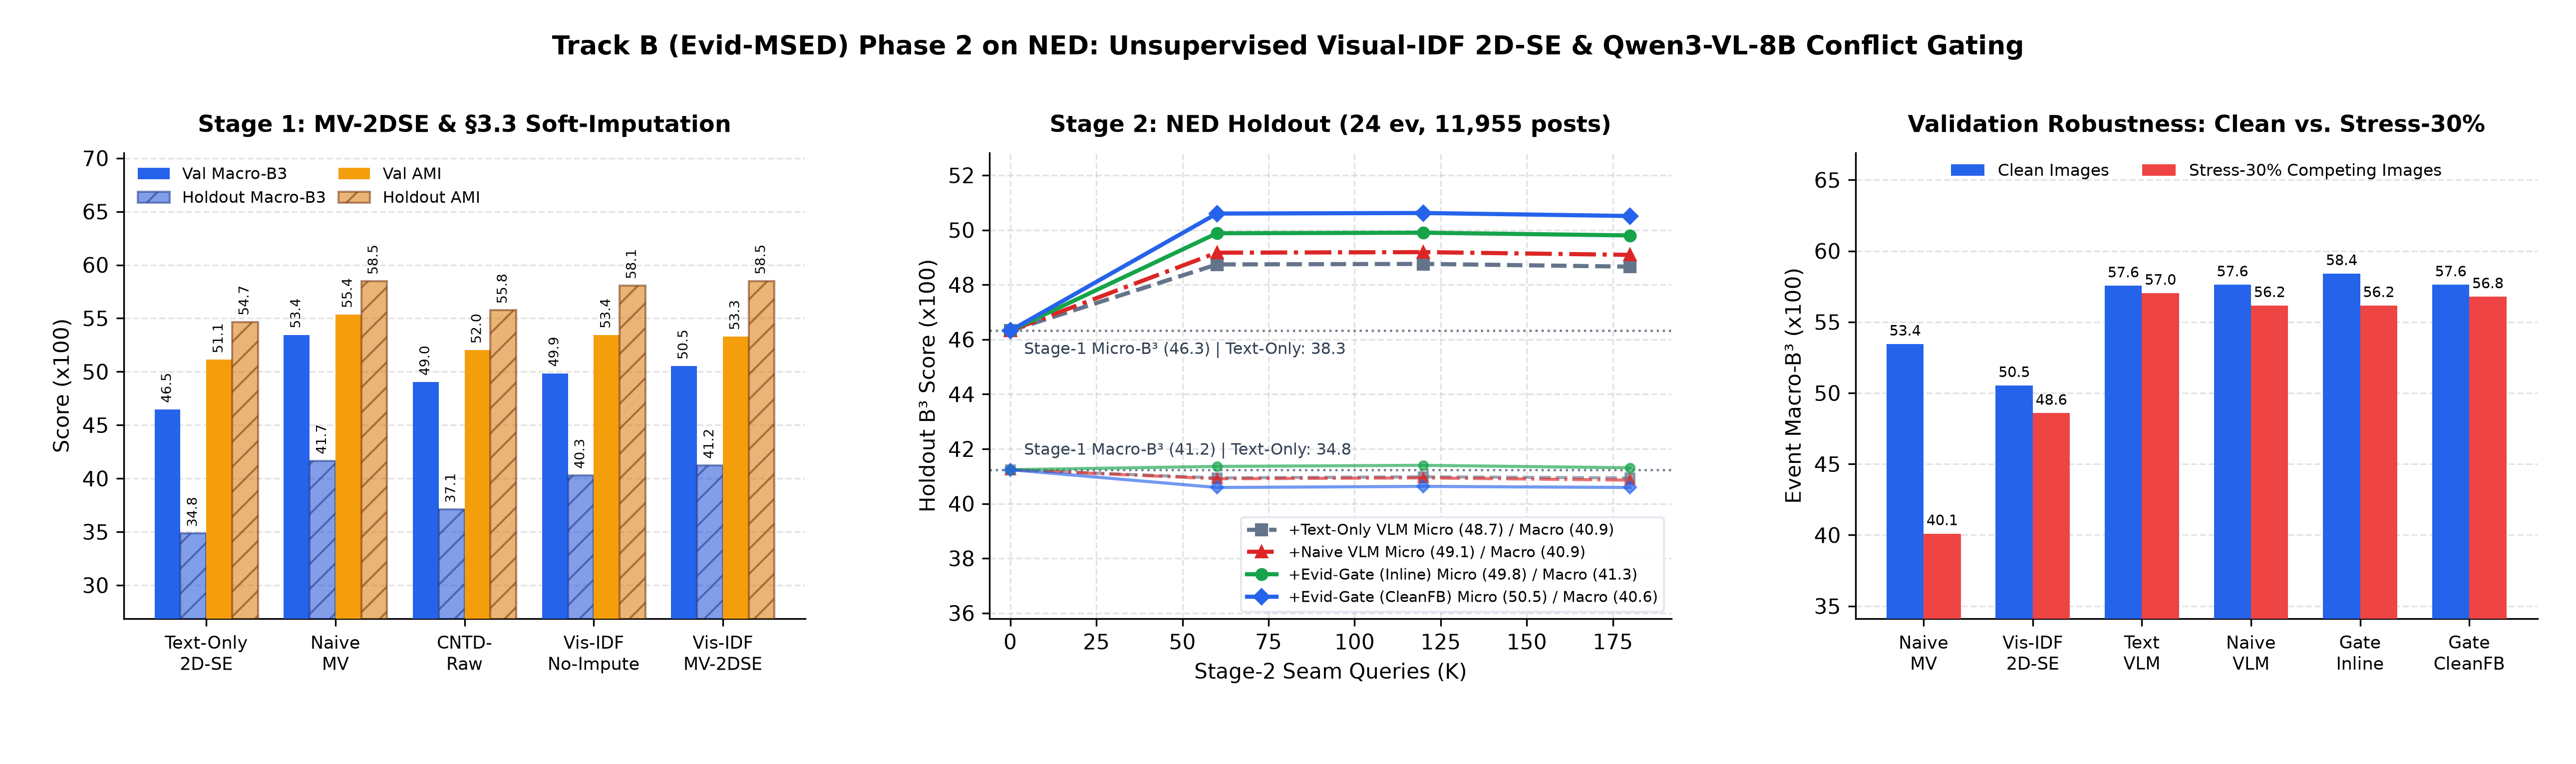
\includegraphics[width=0.98\textwidth]{figures/trackB_phase2_ned_val_holdout.png}
  \caption{Phase~2 evaluation summary: (left) Stage-1 MV-2DSE \& §\ref{sec:stage1_method} soft-imputation ablations across \texttt{Validation} and \texttt{Holdout}; (middle) Stage-2 budget trajectory ($K \in \{60, 120, 180\}$) on unseen \texttt{NED Holdout} showing strong Micro-$B^3$ progression alongside concave diminishing returns after $K=60$; (right) Clean vs.\ Stress-30\% robustness on \texttt{Validation}.}
  \label{fig:phase2_main}
\end{figure*}

\subsection{Stage 2: Conflict-Gated Seam Adjudication}
\label{sec:exp_stage2}

Table~\ref{tab:trackb_stage2_ned} and Figure~\ref{fig:phase2_main} summarize Stage~2 across Clean and Stress-30\% regimes (note \texttt{evid\_comp\_gate\_clean\_fallback} produced identical metrics to \texttt{evid\_self\_gate\_clean\_fallback} because all gated multimodal decisions already satisfied $\text{conf} \ge 0.70$):

\begin{itemize}
    \item \textbf{Clean Supremacy and Leverage:} On \texttt{Validation Clean} ($K=60$), \texttt{Evid-SelfGate (Inline)} wins across every metric---lifting AMI to $0.5748$, Macro-$B^3$ to $0.5841$ ($+7.87\text{ pp}$ over Stage~1, $+11.94\text{ pp}$ over text-only 2D-SE), Micro-$B^3$ to $0.5544$, and unqueried leverage to $19.45$ posts/call ($+1{,}167$ net improved posts vs.\ $13.25$ for \texttt{Naive VLM}). On \texttt{Holdout Clean}, \texttt{Evid-SelfGate (Inline)} is the only policy improving over Stage~1 across all aggregate metrics at both $K=60$ (AMI $0.5877$, Macro-$B^3$ $0.4136$, Micro-$B^3$ $0.4988$, ARI $0.4913$, $24.63$ Fix/Q vs.\ $12.77$ for \texttt{Naive VLM}) and $K=180$ ($4.82$ vs.\ $0.86$ Fix/Q---$5.6\times$ blind VLM efficiency---by rejecting $27.22\%$ of conflicted/non-discriminative seams, preventing $1{,}536$ blind unqueried degradations suffered by \texttt{Naive VLM}). Simultaneously, \texttt{CleanFB} achieves the highest Holdout Micro-$B^3$ ($0.5060$ at $K=60$, $+4.28\text{ pp}$ over Stage~1).
    \item \textbf{Inline Image-Anchoring Under Stress-30\%:} On \texttt{Validation Stress-30\%}, swapped images inside multimodal prompts biased \texttt{Qwen3-VL-8B}'s inline \texttt{same\_event\_text\_only} predictions ($\text{inline\_disagree} = 0$), pulling \texttt{Inline} down alongside \texttt{Naive VLM} ($0.5616$ Macro-$B^3$); image-free fallback (\texttt{CleanFB}) eliminated this anchoring and recovered to $0.5625$ AMI / $0.5678$ Macro-$B^3$ ($18.85$ Fix/Q). Conversely, on \texttt{Holdout Stress-30\%} ($K=60$), \texttt{Inline} achieved top Stress AMI ($0.5605$), Macro-$B^3$ ($0.3778$), ARI ($0.4174$), and $100\%$ merge precision ($1$ TP / $0$ FP), outperforming \texttt{Text-Only VLM} ($0.3595$, hurt by 2 small-event merge errors) by $+1.83\text{ pp}$.
    \item \textbf{Concave Budget Saturation ($K=60$ Peak):} On Holdout Clean, nearly all Stage-2 gains arrive by $K=60$ ($63{,}742$ tokens for \texttt{Inline}), while extending to $K=180$ dilutes per-query Fix/Q from $24.63$ to $4.82$.
\end{itemize}

\begin{table*}[t]
\centering
\caption{Stratified 24-Event Breakdown (\textbf{Small} $<200$ [8 events, $5.8\%$ of posts], \textbf{Medium} $200\text{--}599$ [7 events], \textbf{Head} $\ge 600$ [9 events]) and Stage-2 Executed Action Confusion Matrix on Held-Out \texttt{NED Holdout} ($11{,}955$ posts).}
\label{tab:trackb_strata_ned}
\resizebox{\textwidth}{!}{%
\begin{tabular}{llcccccc}
\toprule
\textbf{Condition} & \textbf{Method} & \textbf{Small $B^3$} & \textbf{Medium $B^3$} & \textbf{Head $B^3$} & \textbf{Macro-$B^3$} & \textbf{Merge TP/FP (Prec.)} & \textbf{Split TP/FP (Prec.)} \\
\midrule
\multirow{6}{*}{Holdout Clean}
& Text-Only 2D-SE (Stage 0) & 0.3326 & 0.3388 & 0.3703 & 0.3485 & --- & --- \\
& Vis-IDF MV-2DSE (Stage 1) & \textbf{0.3753} & 0.4006 & 0.4545 & 0.4124 & --- & --- \\
& + Text-Only VLM ($K=60$) & 0.3270 & \textbf{0.4158} & 0.4777 & 0.4094 & 4/1 (0.8000) & 5/3 (0.6250) \\
& + Naive VLM ($K=60$) & 0.3265 & 0.4135 & 0.4790 & 0.4091 & 2/2 (0.5000) & 5/3 (0.6250) \\
& + \textbf{Evid-SelfGate (Inline, $K=60$)} & 0.3272 & 0.4157 & 0.4887 & \textbf{0.4136} & 4/2 (0.6667) & 5/3 (0.6250) \\
& + Evid-SelfGate (CleanFB, $K=60$) & 0.2905 & 0.4157 & \textbf{0.5008} & 0.4059 & 5/2 (0.7143) & 5/3 (0.6250) \\
\midrule
\multirow{6}{*}{Holdout Stress-30\%}
& Naive MV-2DSE (Stage 1) & 0.3151 & 0.3025 & 0.3792 & 0.3355 & --- & --- \\
& Vis-IDF MV-2DSE (Stage 1) & 0.3564 & 0.3269 & 0.4352 & 0.3773 & --- & --- \\
& + Text-Only VLM ($K=60$) & 0.2972 & \textbf{0.3273} & \textbf{0.4400} & 0.3595 & 3/2 (0.6000) & 15/3 (0.8333) \\
& + Naive VLM ($K=60$) & 0.3567 & 0.3272 & 0.4357 & 0.3777 & 0/0 (0.0000) & 15/3 (0.8333) \\
& + \textbf{Evid-SelfGate (Inline, $K=60$)} & \textbf{0.3567} & 0.3272 & 0.4359 & \textbf{0.3778} & \textbf{1/0 (1.0000)} & 15/3 (0.8333) \\
& + Evid-SelfGate (CleanFB, $K=60$) & 0.3473 & 0.3272 & 0.4358 & 0.3746 & 1/1 (0.5000) & 15/3 (0.8333) \\
\bottomrule
\end{tabular}}
\end{table*}

\begin{figure*}[t]
  \centering
  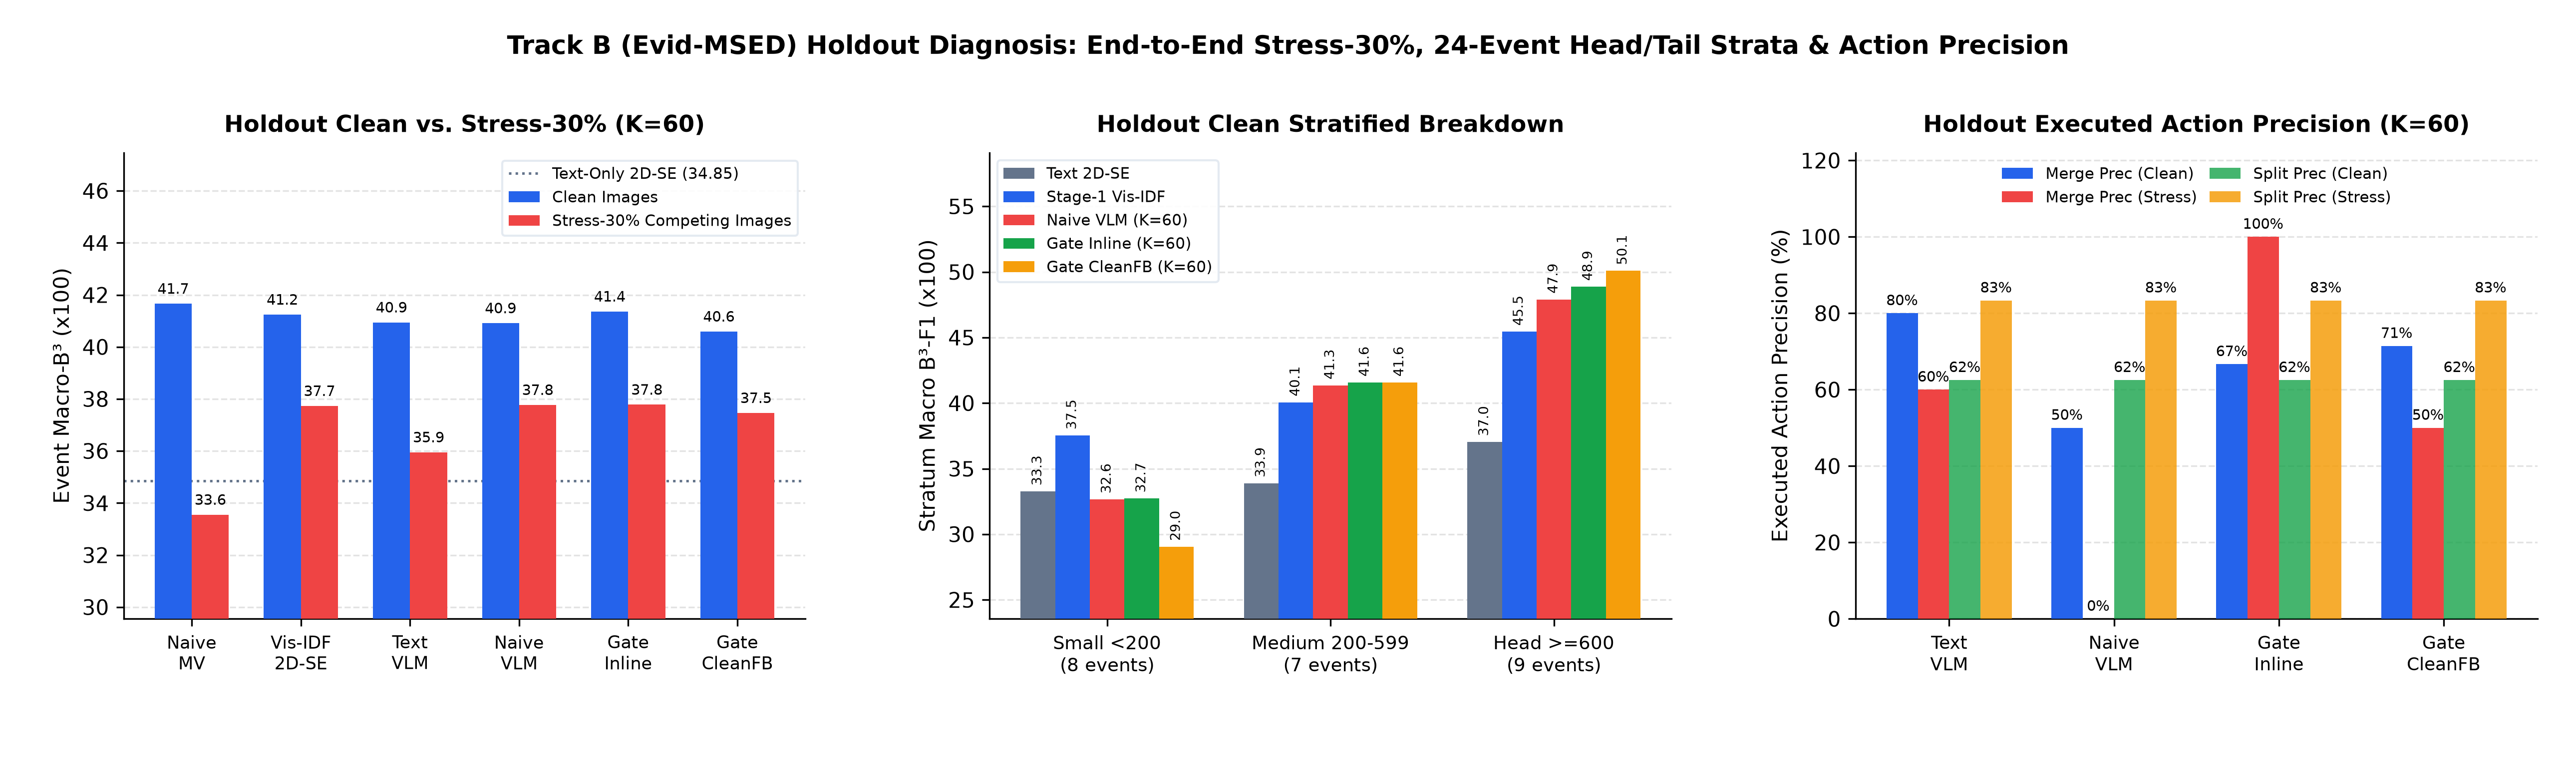
\includegraphics[width=0.98\textwidth]{figures/trackB_phase2_holdout_stress_and_strata.png}
  \caption{Holdout diagnosis ($24$ events, $11{,}955$ posts): (left) End-to-end Clean vs.\ Stress-30\% Macro-$B^3$ at $K=60$; (middle) Clean stratified breakdown showing monotonic Stage~1+Stage~2 gains on Medium and Head events ($0.3703 \to 0.5008$) vs.\ tail erosion from $2$ hard union-find merges; (right) Executed merge and split action precision.}
  \label{fig:holdout_diag}
\end{figure*}

\subsection{Why Micro-$B^3$ Rises While Macro-$B^3$ Plateaus on Holdout}
\label{sec:exp_strata}

Inspecting Stage-2 Holdout numbers superficially might suggest Stage~2 adds little beyond Stage~1 ($\Delta\text{Macro-}B^3 = +0.12\text{ pp}$ for \texttt{Inline}). Table~\ref{tab:trackb_strata_ned} and Figure~\ref{fig:holdout_diag} expose the exact mathematical mechanism:
\begin{enumerate}
    \item \textbf{Large Cumulative Gains on Head and Medium Events:} While Stage~1 elevates all three size strata uniformly (Small $+4.27\text{ pp}$, Medium $+6.18\text{ pp}$, Head $+8.42\text{ pp}$), Stage~2 further pushes Head events ($\ge 600$ posts) from $0.4545 \to 0.4887$ (\texttt{Inline}) and $0.5008$ (\texttt{CleanFB}, $+13.05\text{ pp}$ cumulative over Text-Only), driven by major true merges such as \texttt{E7} ($0.5144 \to 0.7338$, $+21.94\text{ pp}$), \texttt{E4} ($0.4308 \to 0.5552$, $+12.44\text{ pp}$), and \texttt{E37} ($0.3780 \to 0.4641$, $+8.61\text{ pp}$).
    \item \textbf{Two Size-Asymmetric Merge False Positives Erase Tail Weight:} The 8 Small events ($<200$ posts) comprise only $5.8\%$ ($697$) of posts yet carry $33.3\%$ of equal-weighted Event Macro-$B^3$. Although gating increases Holdout Clean merge precision over \texttt{Naive VLM} ($50.0\% \to 66.7\%$ \texttt{Inline} / $71.4\%$ \texttt{CleanFB}), exactly \textbf{two executed \texttt{MERGE} false positives} joined a small cluster into a giant Head cluster ($\text{stratum\_merge\_fp} = \{\text{small}:2, \text{medium}:0, \text{head}:2\}$). Under hard union-find concatenation, absorbing a $<200$-post cluster into a $500$+ post cluster collapses small-event $B^3$ precision (\texttt{E30}: $0.7420 \to 0.3780$ Inline / $0.1654$ CleanFB; \texttt{E18}: $0.4147 \to 0.1488$ Inline / $0.0932$ CleanFB), deducting enough tail points to offset Head gains inside Macro-$B^3$.
\end{enumerate}

\paragraph{Qualitative Stage-2 Seam Cases.}
Real seam logs highlight how explicit gating works on anonymized clusters: (i) \emph{Rescues:} in Validation \texttt{seam\_c32}, two pockets sharing generic \texttt{cnn} tokens split accurately when \texttt{Qwen3-VL-8B} contrasts a Scottish independence vote broadcast against nuclear-victim archival footage ($\text{conf}=1.0$); in Validation \texttt{seam\_c34}, distinct \texttt{\#nepal} emergency contacts vs.\ Google Person Finder screenshots merge cleanly; in Holdout \texttt{merge\_c56\_c90}, Hong Kong street protest schedules and street confrontations unite (\texttt{Text-Only} $= \text{False} \to \text{MM} = \text{True}$). (ii) \emph{Conflict Blocks:} Validation Stress \texttt{seam\_c3} injects a whiskey bottle photo onto sports text ($\text{vis\_conflict} = \text{True}$); Holdout Stress \texttt{merge\_c22\_c103} pairs Sri Lanka blast text with a generic prayer cluster holding a \emph{``Pray for Mexico''} flag---where \texttt{Text-Only VLM} mistakenly merges on generic prayer words while multimodal conflict gating blocks it ($\text{mm} = \text{False}$).
